\documentclass[a4paper,10pt]{article}
%\documentclass[a4paper,10pt]{scrartcl}
\usepackage{graphicx}


\usepackage[utf8]{inputenc}

\title{Estimating reconstruction resolution: SSNR}
\author{Roberto Marabini}
\date{}

\pdfinfo{%
  /Title    ()
  /Author   ()
  /Creator  ()
  /Producer ()
  /Subject  ()
  /Keywords ()
}

\begin{document}
\maketitle

\section{Theoretical Background}

In applied mathematics, the two-dimensional Spectral signal-to-noise ratio (SSNR) measures the normalised cross-correlation coefficient between several two-dimensional images over corresponding rings in Fourier space as a function of spatial frequency (see [1] for details)

\section {Calculation}

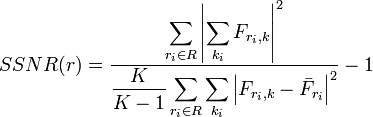
\includegraphics{ssnr.png}

\noindent where $F_{r_{i},k}$ are those pixels of the the Fourier transform of image $k$ at all those pixels placed at radius $r_i$, $F_{r_i}$ are the equivalent pixels computed from the average image. In this form, the SSNR takes many two-dimensional images and converts them into a one-dimensional array. Finally, $K$ is the number of images.

\section {Objetive}
Using Matlab implemented the SSNR as described in [1].

\section {Bibliography}
[1] A new resolution criterion based on spectral signal-to-noise ratios by Michael Unser et al. doi:10.1016/0304-3991(87)90225-7

\end{document}
